%\usepackage{graphicx}

\chapter{Plan}\label{ch:plan}

%Every semester, students ask their supervisor how to write their thesis,
%what the requirements are, and what to write in it.  
%This document tries to answer all such questions.

\section{Our System}

% Image Example
% Need to fix how the diagram is displayed (Also may need to reduce the size of pictures)
\begin{figure}[bp!]
\centering
\graphicspath{{images/} }
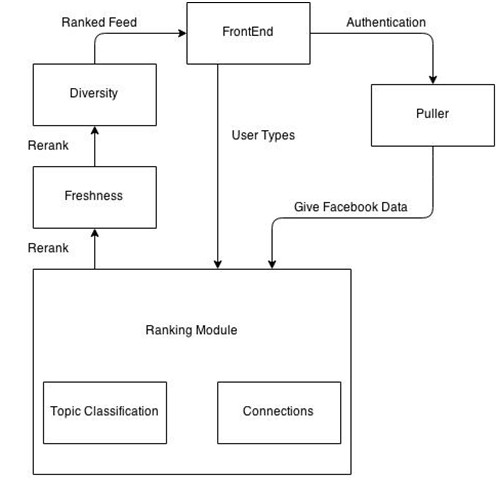
\includegraphics[scale=0.5]{blockdiagram.jpg}
\caption{Block diagram}
\end{figure}

Figure 4.1 provides a general overview of our implementation plan. It is a block diagram of our system. 

\section {Evaluation}

We considered two different ways of evaluating our system.

The first method was to simulate real users by creating Facebook accounts and attempting to mimic behaviour of each user type. We would then create a ground truth regarding how that type of user would like their feed ranked and compare the output of our ranking algorithm to the ground truth. We found quite a few flaws in this method, the major one being how difficult it would be to simulate a real user. Creating social interactions and simulating connections between users would prove very difficult. On top of this, the ground truths that we would be creating could be affected by confirmation bias. This left us with a very questionable evaluation method, so we arrived at our second one.

The second, and chosen evaluation method takes the form of gathering real users and performing a form of usability test. In this test, we will ask participants to order their feeds how they would like it to be seen, this forms an unbiased ground truth. We then run our ranking algorithm on their feeds and compare the ground truth they gave us earlier to the output. In addition to this ground truth comparison, we will ask the user to compare our ranking algorithm with the one provided by Facebook, without telling them which is which. This will give us some subjective results as to whether our ranking algorithm has succeeded in personalising the user's feed.